\chapter{Methodology}
\label{methodology}
\begin{itemize}
    \item Explain the data collection step, and how the comments were collected and aligned using BinSwarm. 
    \item Explain the deduplication methods used and why duplicates in this task are fine, but why we choose to report the deduplicated results anyway.
    \item Explain the experimental setup for the standard model, how we pre-processed the data, fed it into the model and the evaluation 
    \item Explain the experimental setup for the pre-training, the translation, DOBF and span detection, how and why the pre-training steps were done, and how they were evaluated
    \item Explain the manual evaluation of the stripped code
\end{itemize}
\newpage

\section{Data Collection}
To create a large and diverse dataset to train and assess our solution we made use of BinSwarm \cite{InlinedFunc}, an existing dataset of aligned decompiled and stripped decompiled functions \footnote{BinSwarm; \url{https://hub.docker.com/r/binswarm/cbuilds}}.

Buildswarm starts by collecting C-based projects from Github. The projects are filtered to only include projects that are: Actively being developed, using Travis CI and built for Ubuntu Linux. The projects are then built using Docker. The resulting binaries are then stripped and both the stripped and unstripped binaries are decompiled using Ghidra, the functions are extracted and aligned with the source code. A high level overview of this process can be found in figure \ref{fig:dataCollection}.

\label{fig:dataCollection}
\begin{figure}[!h]
  \centering
  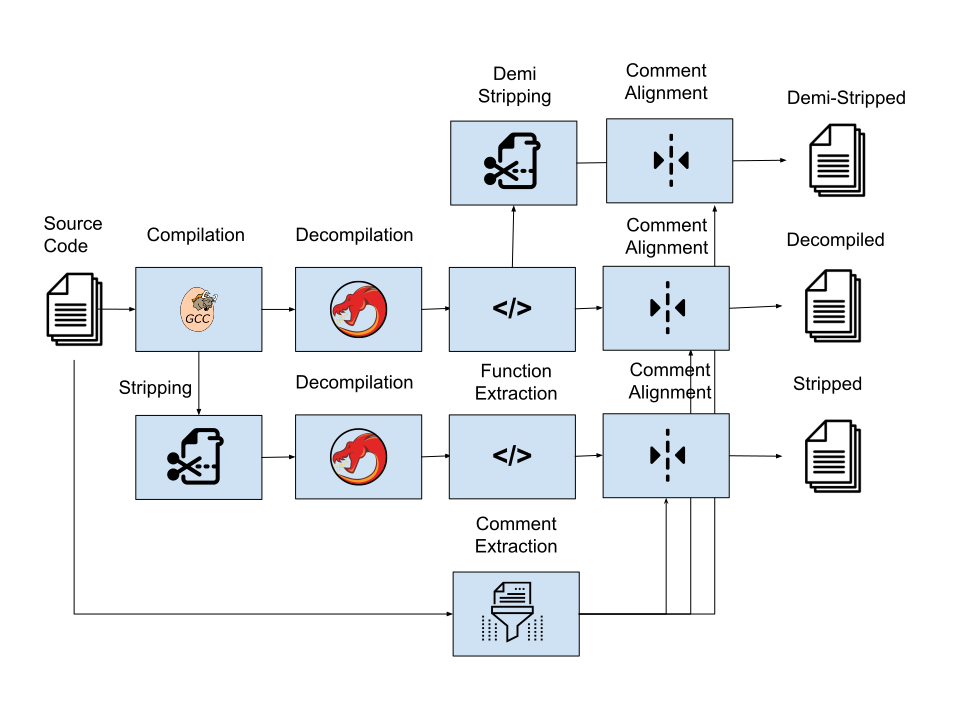
\includegraphics[width=\linewidth]{img/dataCollection.png}
  \caption{Data Collection}
\end{figure}

From the dataset of decompiled functions another dataset is also created. We can emulate the process of stripping by removing all the identifiers from the decompiled code and replacing them with placeholders, for the purpose of clarity, we call this demi-stripped data. Like the stripped dataset, the identifiers are all removed, but the decompiler still had access to the identifiers and could use the symbol table during decompilation. Most importantly, this demi-stripped dataset still has the same structure and control flow as the unstripped decompiled dataset.

\section{Dataset Split}
The dataset is split into a train, test and validation set. These sets constitute approximately, 80\%, 10\% and 10\% respectively\cite{recommend_summarization} of the complete dataset. To prevent leakage of vocabulary and code patterns between the sets, we sample the sets in a cross-project manner. Meaning that an entire project gets assigned to one of the sets, and functions from the same project cannot be assigned to different sets. The different sets should also have a similar distribution of optimization level and average source length.

\section{Duplication}
Large corpora of code, like the corpus gathered by BinSwarm, tend to have a high degree of duplication \cite{leclair_recommendations}. Snippets of code that are relatively unchanged appear in multiple parts of the corpus. This can be in the form of functions that are copied, generic or auto-generated. These functions will then appear in multiple repositories and might be duplicated across the training and testing data.

The issue with code duplication in classical code summarization is that the models and tools are supposed to be used to generate summaries for new and unseen code. The evaluation metrics should therefore measure the generalization of the tool on new samples \cite{allamanis_adverse}. The usecase outlined in this work, is however, more akin to deobfuscation. Compiled code contains a lot of duplicate code, and understanding this code is still difficult and of importance towards the understanding of the binary. We will therefore focus on the performance of the model on code with duplicates, but we will also report the deduplicated results.

\section{Fine-Tuning}
We fine-tune a pre-trained CodeT5-base model on the constructed dataset. The model is trained on the summarization task as defined in the model. The model is trained on the train set, then evaluated after every epoch on the validation set and finally tested on the test set. The performance of the model is measured using the EM (exact match), BLEU-4 scores.

\section{Pre-Training}
To apply and assess other pre-training objectives we train a CodeT5-base model on a predefined objective, then after that pre-training step, we fine-tune the resulting model on our fine tuning datasets. We essentially apply another pre-training step to the already pre-trained base model. We can then measure the impact of the pre-training step on the performance of the model after fine-tuning.

\label{fig:preTraining}
\begin{figure}[!h]
  \centering
  \includegraphics[width=\linewidth]{img/pre-training.png}
  \caption{Pre-Training}
\end{figure}

